Some energy models do not seek to accurately rank potential conformations, fast ``screening'' functions attempt to quickly differentiate physically impossible conformations from plausible conformations without performing an expensive minimization or energy calculation step.
Application of these screening functions has the potential to greatly reduce the number of potential conformations that must be scored using the full detail energy function, greatly decreasing the overall cost of conformation prediction.
These screening criteria can be applied either during the sampling procedure, potentially eliminating sampling of a large area of excluded conformation space, or after sampling before a more expensive energy function is applied to rank conformations.
Effective screening criteria have a large impact on the total performance of a structure prediction method.

One of the earliest screening criteria was the hard sphere overlap collision detection \cite{levinthal1966molecular}, and this method is consistently included in screening scriteria.
Other screens include:
\begin{enumerate}
\item bounds on bond lengths and angles, as a single bond which deviates significantly from equilibrium can dominate the energy of a conformation,
\item limitations on $\phi$-$\psi$ space occuped by backbone dihedrals corresponding to the Ramachandran plot of the residue,
\item limiting side chain dihedrals to staggered conformations, which correspond to the low energy well of side chain dihedral space \cite{moult1986algorithm},
\item excluding structuctures which present excessive solvent accessible surface area, as this conflicts with the hydrophobic effect, which has a large effect on the conformation of the native state \cite{chothia1975principles}
\item limitations on the number of ``dry'' cavities, and the number of internal charged residues \cite{moult1986algorithm}
\end{enumerate}

\subsection{The General Form of the Energy Model}
\label{subsection:energy_general_form}
The general form of most molecular mechanics energy potentials is reasonably consistent, with bonds and angles being modeled as a spring, dihedrals as a Fourier series.
\begin{equation}
E \left(r^N \right ) = E_\mathrm{bonds} + E_\mathrm{angles} + E_\mathrm{dihedrals} + E_\mathrm{nonbonded}
\label{equation:opls}
\end{equation}

\begin{equation}
E_\mathrm{bonds} = \sum_\mathrm{bonds} K_r (r-r_0)^2
\end{equation}

\begin{equation}
E_\mathrm{angles} = \sum_\mathrm{angles} k_\theta (\theta-\theta_0)^2
\end{equation}

\begin{equation}
E_\mathrm{dihedrals} = \sum_{i=1\dots4} {\frac {V_i} {2} \left [ 1 + \cos \left ( i * (\phi-\phi_0) \right ) \right ] }
\end{equation}

The non-bonded terms are modeled as a Columbic potential between any point charges and a Lennard-Jones or 6-12 potential between any non-bonded atoms.
These non-bonded atoms are phased in by a ``fudge factor'' for atoms in a 1-4 configuration.
\begin{equation}
\begin{split}
E_\mathrm{nonbonded} = \sum_{i>j} f_{ij} 
                \left (
                        \frac {q_i q_j e^2}{r_{ij}}
                    + 4 \epsilon_{ij} 
                    \left  [  
                        \left ( \frac{\sigma_{ij}}{r_{ij}}\right )^{12}
                      - \left ( \frac{\sigma_{ij}}{r_{ij}}\right )^{6}
                    \right ]
                \right )
\\
f_{ij} = 
  \begin{dcases*}
   0    & if $i$ and $j$ are separated by 2 or fewer bonds\\
   0.5  & if $i$ and $j$ are separated by 3 bonds\\
   1.0  & otherwise
  \end{dcases*}
\end{split}
\end{equation}

Where $\sigma_{ij} = \sqrt{\sigma_{ii} \sigma_{jj}}$ and $\epsilon_{ij} = \sqrt{\epsilon_{ii}\epsilon_{jj}}$ \cite{jorgensen1996development}.


\subsection{Molecular Surfaces}
\label{subsection:molecular_surfaces}
Central to the discussion of solvent is a discussion of how to formulate the surface of a protein.
The most frequently used formulations of surface area include the Van der Waals (VDW) surface, the solvent accessible surface, and the Connolly surface (also known as the molecular surface).
\begin{figure}[h]
\centering
\begin{subfigure}[b]{0.4\textwidth}
\centering
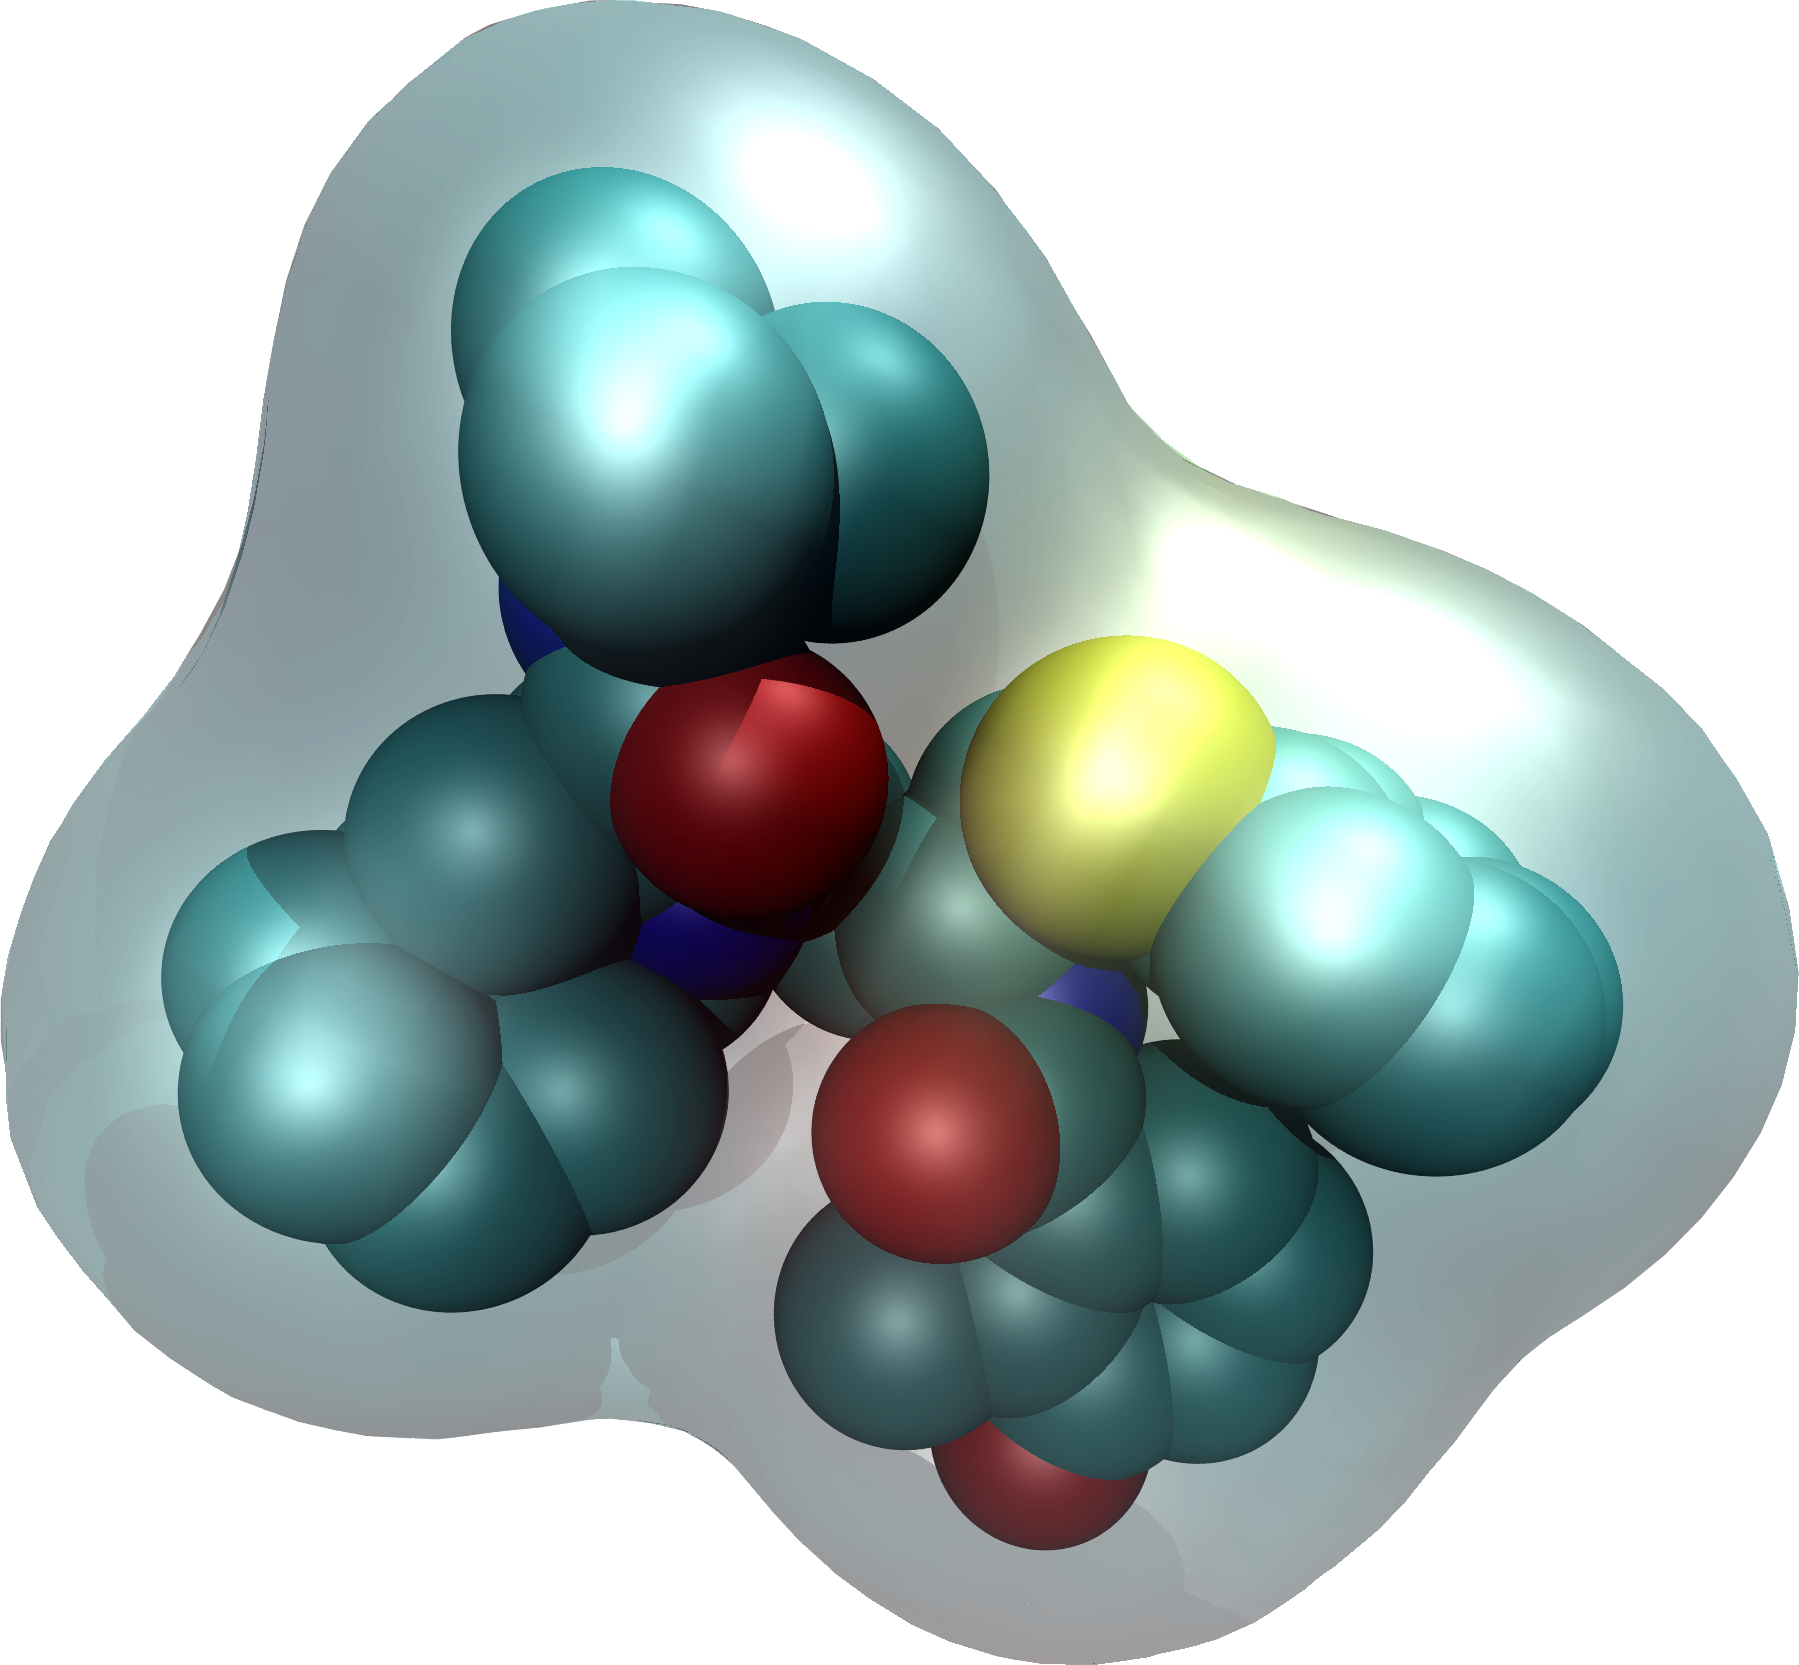
\includegraphics[width=\textwidth]{figures/vdw.png}
\caption{}
\label{figure:vdw_surface}
\end{subfigure}
\hspace{0.1\textwidth}
\begin{subfigure}[b]{0.4\textwidth}
\centering
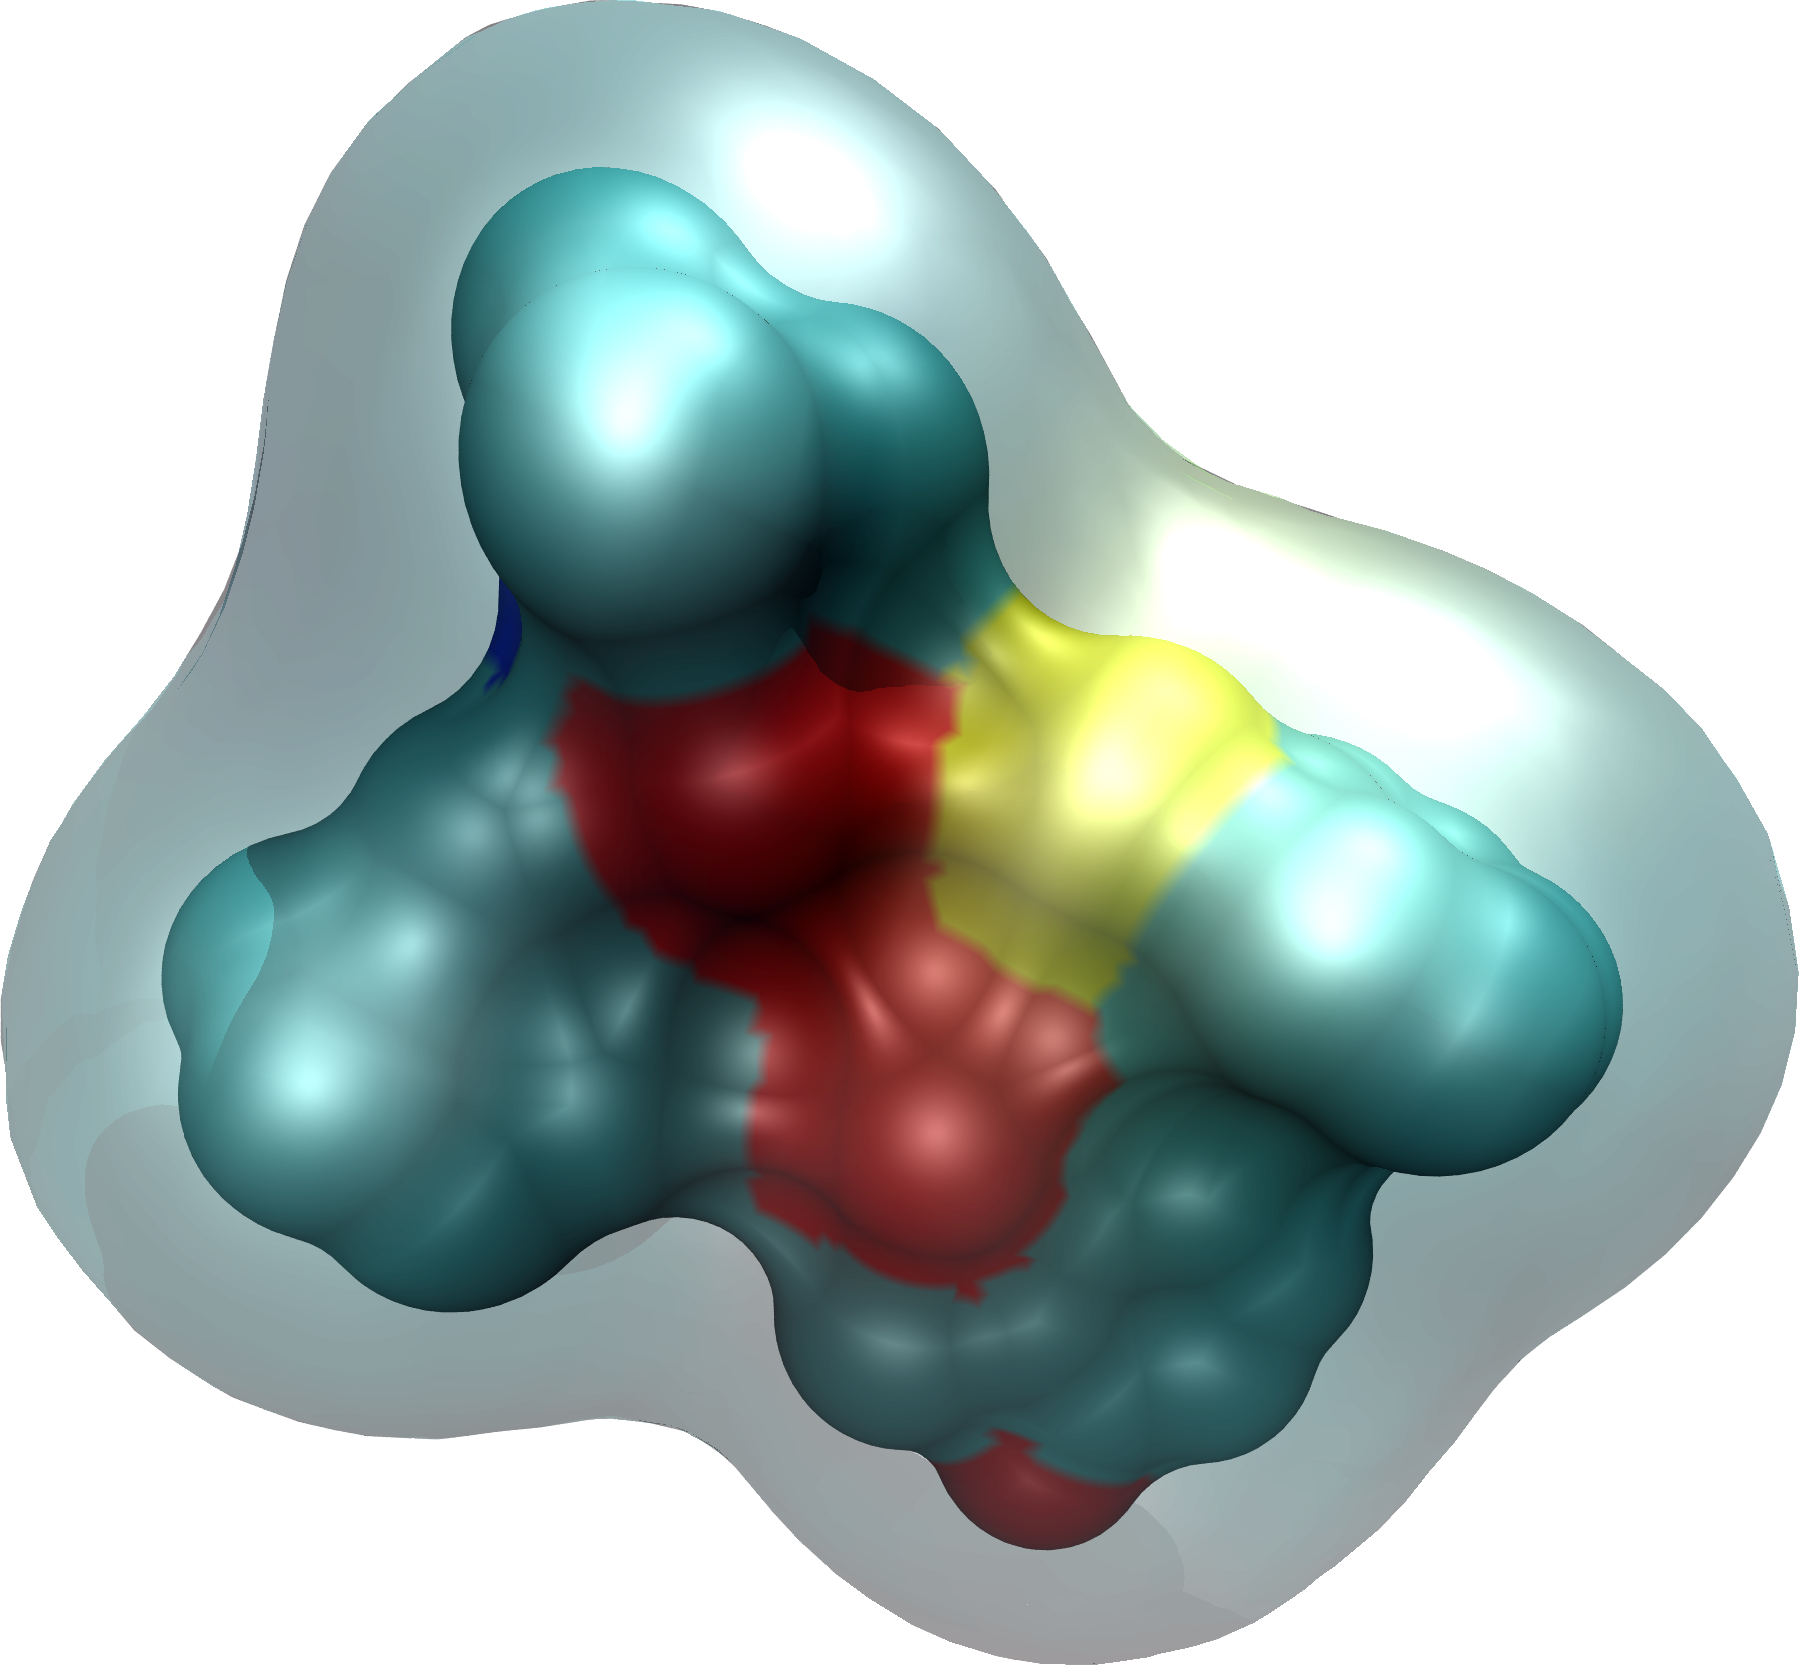
\includegraphics[width=\textwidth]{figures/molecular.png}
\caption{}
\label{figure:molecular_surface}
\end{subfigure}
\caption{(a) The Van der Waals surface of Nelfinavir, defined by the surface of the volume excluded by the VDW radii of the atoms in the structure.
(b) The molecular surface, defined as the surface of the volume excluded from a probe of 1.4 angstroms (the radius of a water molecule).
Both surfaces are enclosed by an approximate solvent accessible surface, which is defined as the surface traced by rolling a spherical probe over the VDW surface.
Figure generated using Nelfinavir structure from PDBid 3EL5 \protect\cite{king2012extreme}, and using VMD and POV-Ray \protect\cite{humphrey1996vmd,povray}.}
\label{figure:surfaces}
\end{figure}
\begin{enumerate}
\item The Van der Waals (VDW) surface is the surface formed by the VDW radius of each molecule, though the exact radii mayy vary in different energy functions.
Frequently the VDW radii are scaled down in order to reduce the effect of steric clashes and help generate more initial structures \cite{schulz2003binding,halgren2004glide}.
Clashes which are tolerated using these scaled down radii can later be resolved in minimization.
This is illustrated in figure \ref{figure:vdw_surface}.
\item The solvent accessible surface, which is defined as the surface traced by the center of a spherical probe ``rolled'' over the VDW surface \cite{richards1977areas}.
This idea is very closely related to the idea of the solvent excluded volume, or the shape of the solvent cavity enforced by the VDW surface of the molecule \cite{richmond1984solvent}.
An illustration of the solvent accessible surface is shown enclosing both a VDW and molecular surface in \ref{figure:surfaces}.
\item The molecular surface, or Connolly surface, is composed of the VDW surface in areas where the spherical probe touches the VDW surface, in union with all points on the probe ``between'' two points on the VDW surface when the probe is contacting multiple atoms \cite{connolly1983analytical} -- put another way, the surface of the volume which intersects no possible probe location.
This is shown in \ref{figure:molecular_surface}
\end{enumerate}
Frequently, these surfaces are approximated numerically, using the Shrake-Rupley algorithm \cite{shrake1973environment}, by considering a spherical mesh about every atom and including only points that satisfy the definition of the surface, or using these points to interpolate a surface.

The effect of surface area on determining protein structure is determined by physical forces.
However, the significance of the effect of surface area is well illustrated by the observation that the ratio of total area of a theoretical unfolded, i.e. linearly arranged, protein to its length is almost among proteins, only varying by \textapprox3\% between different proteins.


\subsection{Solvent Models}
\label{subsection:Solvent Models}
Beyond covalent terms and electrostatic effects, solvation effects have a very large effect on protein structure, and the interactions between proteins and small molecules.
Therefore it is critical to accurately model the effect of the solvent on the molecule.
While explicitly modeling each water molecule and sampling over possible conformations is the most realistic possible model, doing so requires calculating both a large number of solute-solute interactions as well as sampling extensively different solvent configurations.
In this case it is likely that more time will be spent determining the behavior of the solvent than that of the solute.
Because of these complexities even with efficient methods of sampling explicit solvent models, these simulations are too expensive to use on systems the size of proteins \cite{figueirido1997large,zhang2001solvent}.

Therefore there is significant interest in continuum models which accurately describe the mean force of water, without requiring additional sampling or interactions as in explicit models \cite{zhang2001solvent,still1990semianalytical,qiu1997gb}.
These methods have the potential to be three orders of magnitude, or even more, faster than explicit solvent experiments, and a number of different methods have been shown to accurately describe solvent effects \cite{zhang2001solvent}.

The total free energy of solvation can be separated into polar and non-polar components, which correspond to the work done inserting the uncharged solute molecule, or protein, into the solvent and then building the charges to their native values \cite{roux1999implicit}.
\begin{equation}
E_{\mathrm solvent} = {\Delta}W_{\mathrm non-polar} + {\Delta}W_{\mathrm electrostatic}
\end{equation}

According to scaled particle theory the non-polar work done by inserting a sphere into a solvent can be approximated if the raidus of the sphere is neither too large nor to small as
\begin{equation}
{\Delta}W_{np}(s) = \gamma SA(X)
\end{equation}

where $\gamma$ is the surface tension of the solvent and the surface area corresponds most closely to the Connolly surface.

The electrostatic contribution to the solvent energy is the work necessary to add a charge to a hard sphere atom already in the solvent.
The charge density in the solvent can be given by the Poisson-Boltzmann equation
\begin{equation}
\nabla \cdot \left [ \epsilon(r) \nabla\psi(r) \right ] = -4\pi\rho_{u}(r)
\end{equation}

Though it is possible to solve this at every step of a simulation, it becomes rather expensive, therefore faster approximations are sought \cite{nicholls1991rapid}.
The total work can be approximated by the Born model
\begin{equation}
{\Delta}W_{electrostatic} = \frac{Q^{2}}{2R} \left ( \frac{1}{\epsilon_{v}} - 1 \right )
\end{equation}

However, this assumes that the induced charge in the solvent is entirely concentrated on the surface of the ion, which is impossible, therefore $R$, or the Born $\alpha$ radius becomes a fit parameter, representing the effective radius of a charged sphere in the solvent.

The electrostatic solvation contribution can also be expressed as
\begin{equation}
{\Delta}W_{electrostatic} = 
\frac{1}{2} \sum_{i,j}q_{i}q_{j}f(x_{i},x_{j}) = 
\frac{1}{2} \sum_{i}q^{2}_{i}f(x_{i},x_{i}) + \frac{1}{2} \sum_{i \neq j}q_{i}q_{j}f(x_{i},x_{j}) 
\end{equation}

where f is a weighting function for the interaction between charges $q_i$ and $q_j$.
Historically there are a variety of methods of approximating this weighting function, however one of the most popular is the generalized Born (GB) \cite{still1990semianalytical}.
In the generalized Born approch
\begin{equation}
f(x_i,x_j) = \sqrt{
                    d(x_i,x_j) +
                    R_i R_j e^{\frac{-d(x_i,x_j)^2}{4 R_i R_j}}
                  }
\end{equation}

and one of the limiting factors to accuracy becomes obtaining proper estimates of the effecitve radii, since charges are not uniformly exposed to the solvent \cite{schaefer1996comprehensive}.

Another approach is to estimate both the nonpolar and electrostatic contributions to solvation as proportional to the surface area, with different proportionality constants for different atoms.
\begin{equation}
{\Delta}W = \sum_{atoms}\gamma_{atom}SA(atom)
\end{equation}

Although this method is very inexpensive to compute, it can be somewhat difficult to solve for the force on an atom, due to the way the surface changes as atoms move \cite{roux1999implicit}.

